\documentclass{article}
\usepackage{ctex}
\usepackage{graphicx}
\usepackage{amsmath}
\usepackage{float}

\title{OSTEP笔记}
\author{trailblaer887}
\date{2026年2月24日}





\begin{document}
\maketitle
\tableofcontents
\section{Visualization(CPU)}

\subsection{Mechanism: Limited Direct Execution}
即``有限制地"将进程放在CPU上直接执行.为了使这个机制正常工作,我们需要解决两个问题
\begin{enumerate}
    \item Restricted Operations \\
    为了保障系统安全,不能允许进程直接进行操作(读写I/O或申请CPU资源等``敏感操作"),因此我们用``分权"将进程和``敏感操作"隔离开,统一交给神圣的``操作系统"来管辖:设置\textbf{user mode}和\textbf{kernel mode},将进程能干的事限制在安全范围之内.你说你想读写I/O?问问操作系统吧! \\
    接着,OS,hardware,process,合作进行``敏感操作""(详细过程见本章中的流程图)
    
    \item Switching Between Processes \\
    进程切换方式分为\textbf{Cooperative Approach}和\textbf{Non-Cooperative Approach}.简单来说,前者靠进程自觉让出CPU控制权,假设每个进程都守规矩;而后者为了防止有心者恶意占用CPU资源,便设置\textbf{timer interupt}强制进程让出CPU以便给其他进程机会运行. \\
    进程切换也包括\textbf{上下文切换}(\textbf{context switch}).容易让人困惑的是,当实现进程A切换至进程B时,首先先将进程A的相关信息(registers,PC等)保存至hardware的每个进程相关kernel stack中,然后OS再将kernel stack中的信息转移至PCB中的相关部分,返回时过程类似,需重点理解.
\end{enumerate}

\subsection{Scheduling: Introduction}
\begin{enumerate}
    \item Scheduling Metrics \\ 
    Scheduling metrics有两大死对头：turnaround time和response time。要想平衡两者很困难（trade-off的艺术），由此也派生出两类调度方法（这里暂且认为每个进程的用时一致，即“上帝视角”）。
    \item Good for Turnaround Time \\
    其代表为\textbf{FIFO}(first in, first out)和\textbf{SJF}(short job first)(具有抢占式特点的则叫\textbf{STCF}(short time-to-completion first)或\textbf{PSJF}(preemptive shortest job first))。
    \item Good for Response Time \\
    其代表为\textbf{RR(Round Robin) scheduling}或\textbf{time-slicing}
    \item Incorporating I/O
    如果考虑I/O操作的话，我们可以使用\textbf{Overlap}思想，在一个进程执行I/O操作时，CPU去执行另外一个进程，提高CPU的利用率，同时减少时间浪费。
    \item No More Oracle \\
    但是我们并不是“上帝”，并不能提前知道一个进程总共要花费多长时间，SJF等方法就失效了。如何克服这个问题呢？在下一节我们会建立一个新的scheduler——\textbf{它能根据过去来预测未来}，也被称为\textbf{multi-level feedback queue}。
\end{enumerate}

\subsection{Scheduling: The Multi-Level Feedback Queue(MLFQ)}
\begin{enumerate}
    \item Basic Concept \\
    我们将进程分为两类:
    \begin{itemize}
        \item \textbf{Short-running}利用CPU较少，主要时间花费在I/O操作上（主要是交互型任务）。
        \item \textbf{Long-running}大量利用CPU，很少有I/O操作（例如批处理任务等）。
    \end{itemize}
    \textbf{MLFQ}构建多个具有不同优先级的队列，并在基础上进行调度，文中模拟了一个\textbf{简单的scheduler}，并不断优化以缓解\textbf{Stavation},\textbf{Security},\\
    \textbf{Behavior Changes}问题，其遵循以下规则：
    \begin{enumerate}
        \item 处于高优先级的进程优先执行，具有相同优先级的进程进行\textbf{RR scheduling}。
        \item 当一个进程进入调度范围，首先会被放在最高优先级队列中。
        \item 当某个进程在某个队列中被调度了一定的的CPU处理时间(看\textbf{时间的积累量}，不管是否中间有过I/O操作)，如果其值超过一定的阈值(\textbf{allotment})，就下调其优先级。
        \item 当经过一段时间$S$时，将全部进程的优先级提至最高。
    \end{enumerate}
    \item Reality
    实际上基于MLFQ的scheduler及其变体百花齐放啊，很多OS都在用，也有很多其他的调度策略（如\textbf{decay-usage}等）。同时管理者的提示（\textbf{advice}）也时很有用的，可以用\texttt{nice}来手动调整优先级，
    毕竟哪个进程优先，管理者心里有杆秤，也免了OS猜了。
\end{enumerate}
\subsection{Scheduling: Proportional Share}
\begin{enumerate}
    \item Basic Concept \\
    本章介绍了三种scheduling method: 
    \begin{itemize}
    \item \textbf{lottery scheduling}，具有随机性
    \item \textbf{stride scheduling}，具有决定性，stride和lottery成反比
    \item \textbf{complete fair scheduler}，以\textbf{virtual runtime}\texttt{(vruntime)}为标准，
    设置优先级，转换为权重计算\texttt{vruntime}，动态时间片
    \begin{equation*}
        \texttt{time\_slice}_{k} = \frac{\texttt{weight}_{k}}{\sum_{i=0}^{n-1} \texttt{weight}_{i}} \cdot \texttt{sched\_latency}
    \end{equation*}
    \begin{equation*}
        \texttt{vruntime}_{i} = \texttt{vruntime}_{i} + \frac{\texttt{weight}_{0}}{\texttt{weight}_{i}} \cdot \texttt{runtime}_{i}
    \end{equation*}
    \textbf{如何快速查找/添加减少“运行进程队列”里的成员呢？} \\
    用\textbf{红黑树}数据结构，善用数据结构减少payload也是scheduling method重要的一环！
    \end{itemize}
\end{enumerate}

\section{Visualization(Memory)}
\subsection{The Abstraction: Address Spaces} 
有三个目标：\textbf{transparency}, \textbf{efficiency}, \textbf{protection}
\subsection{Interlude: Memory API}
本章简要介绍了\texttt{Memory API},以及有关的内存问题。
\subsection{Mechanism: Address Translation}
介绍了"base-and-bounds"方法来翻译虚拟地址（听听就好，已经过时了）,指出了硬件支持的重要性，介绍了地址翻译的简化版
\subsection{Segmentation}
用两个寄存器还是太少了（大量sparse space仍在内存中）。为了解决这个问题，我们使用\textbf{段寄存器}，同时有利于code sharing（这里要设置protect bit）
\begin{enumerate}
    \item \textbf{两种分段模式}
    \begin{itemize}
        \item Fine-grained（分很多段），用内存中的\textbf{segment table}存段的物理地址
        \item coarse-grained（分少量段）
    \end{itemize}
    \item \textbf{管理Free space} \\
    内存中存在external fragmentation和internal fragmentation
    为了减少external fragmentation，可以使用以下两种方法：
    \begin{itemize}
        \item Capacted memory 将物理内存井然有序整理一下，缺点是运行时时间开销大
        \item free-list management algorithm 就是用链表把空闲内存串起来，分配时按一定标准分配，有以下标准
            \begin{itemize}
                \item best-fit
                \item worst-fit
                \item first-fit
                \item \dots
            \end{itemize}
        其实有很多中算法，可以自行了解。
    \end{itemize}
    \end{enumerate}
\subsection{Free-Space Management}
\subsubsection{Assumptions}
\begin{itemize}
    \item basic interface: \texttt{malloc()}和\texttt{free()}
    \item 我们关注\textbf{external fragmentaion}
    \item 一旦一段内存被分配，就不能再挪动其位置了
    \item allocater管理着连续的字节区域
\end{itemize}
\subsubsection{Low-level Mechanisms}
\begin{itemize}
    \item \textbf{Spliting and Coalescing}
    \item \textbf{Tracking The Size Of Allocated Regions(embedding a free list )}
    \item \textbf{Growing The Heap}
\end{itemize}


\subsubsection{Basic Strategies}
\begin{itemize}
    \item \textbf{Best Fit}
    \item \textbf{Worst Fit}
    \item \textbf{First Fit}
    \item \textbf{Next Fit}
    
\end{itemize}
\subsubsection{Other Approaches}
\begin{itemize}
    \item \textbf{Segregated Lists}：根据\textbf{空闲内存的大小}分成不同的链表，减少搜索时间
    \item \textbf{Buddy System}：将内存分成大小为2的幂次方的块，分配时找到最合适的块，优点是\textbf{分割和合并都很简单}，缺点是可能会有较大的internal fragmentation
\end{itemize}

\subsection{Paging: Introduction}
\textbf{page}: 将内存分割成\textbf{固定大小}的块 \\
\indent \textbf{page table}: 其中每个PTE都存储VPN到PPN的\textbf{映射}和多个\textbf{状态位} \\
\indent \textbf{MMU}: CPU中执行地址翻译的硬件 \\
\indent 核心问题：1. 访问页表太慢 2. 页表占用空间太大

\subsection{Paging: Faster Translations (TLBs)}
由OS处理TLB不命中(将内存中的相应内容放到TLB里，再访问TLB)，同时为了防止\textbf{访存不命中死循环}(跳转到处理访存不命中的地址也需要翻译，而它也不在缓存中时，就会发生死循环)，可以\textbf{直接用物理地址}或\textbf{在TLB中设立常驻有效翻译}(valid = 1，其中\textbf{wired register}告诉硬件为OS保留多少个槽位)。\\
\indent 如果涉及到多个进程，则可以通过\textbf{重置valid = 0}或\textbf{设置address space identifier(ASID)位来区分不同进程的地址空间} \\
\indent \textbf{替换策略}: \textbf{LRU}

\subsection{Paging: Smaller Tables}
上一章，由于频繁访问页表太慢，我们讨论了如何提升翻译的速度。在这一章，鉴于有时页表会占有大量内存，我们将讨论如何如何减少其内存占用。
\begin{itemize}
    \item \textbf{Hybrid Approach: Paging and Segments} \\
    由于这种“混合方法”会使页表的长度“可变”，所以在内存分配方面很容易造成internal Segmentation，而且管理方法较为复杂
    \item \textbf{Multi-level Page Tables} \\
    \textbf{核心思想：对于页表同样以“页”为单位进行分割，再用page directory索引已被分割的页表的每一页(二级)。
    多级则再将page directory按“页”为单位进行分割，以此类推...} \\
    以下为二级页表下虚拟地址的各部分含义：
    \begin{figure}[H]
        \centering
        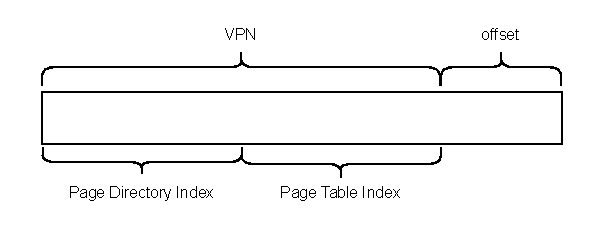
\includegraphics[width=0.9\textwidth]{figures/two_levels_page_tables.pdf}
    \end{figure}
    此时，只有被实际用到的虚拟地址才会分配相应的PTE，有效减少的页表的PTE数量。同时，由于每一级按“页”分割，在内存分配方面也十分方便，
    而且页表在物理内存中也不用必须连续分布了。
    \item \textbf{Inverted Page Tables} \\
    使用哈希表，使\textbf{多个进程仅使用单个页表}，减少内存占用。

\end{itemize}

\subsection{Beyond Physical Memory: Mechanisms}
这一章，我们将\textbf{硬盘}作为虚拟内存的“后备资源”，进一步提高内存的虚拟化，使得程序员无需手动加载文件到内存。
磁盘中有一个\textbf{Swap space}供内存页的\textbf{临时}卸载和加载，PTE中的\textbf{Present bit}表示该虚拟地址的内容在内存中还是在硬盘上。\\
\indent OS中存在\textbf{Hign watermark}(HW)和\textbf{Low watermark}(LW)决定何时该实现\textbf{页面的替换}。当OS注意到可用页面数小于LW时，便启用一个
后台线程(\textbf{swap daemnn/page daemnn})将一批页面换入Swap space，直到可用页面数多余HW(将一批页面统一处理也可以提高硬盘读写的效率)
\indent 以下为地址访问和缺页处理的控制流:
\begin{figure}[H]
    \centering
    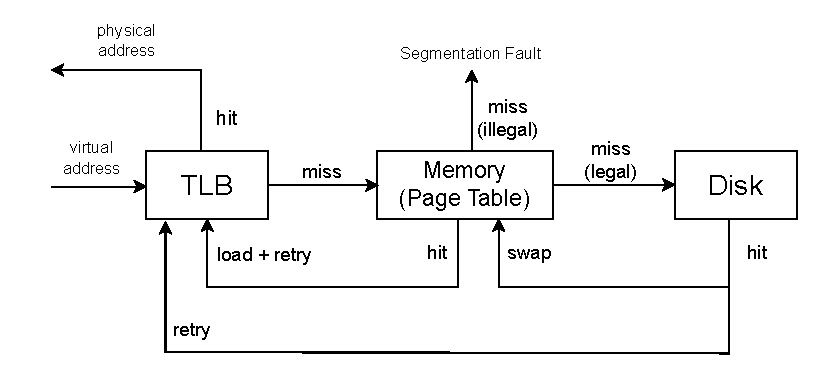
\includegraphics[width=1.0\textwidth]{figures/page_fault_control_flow.pdf}
\end{figure}

\subsection{Beyond Physical Memory: Policies}
本章主要介绍和“页替换算法”及性能判断方法
\subsubsection{Metrics}
平均访存时间公式：
$$
AMAT = T_M + (P_{Miss} \cdot T_D)
$$
\textbf{The Optimal Replacement Policy}：最佳的(也是不切实际的)替换算法(通过未来情况做出判断)。可以将\textbf{现有的替换算法与之相比较}，从而判断当前算法与最优解的差距
\
\subsubsection{Policies}
\begin{itemize}
    \item \textbf{FIFO}
    \item \textbf{Random}
    \item \textbf{LFU}
    \item \textbf{LRU} \\
    它和LFU一样，是\textbf{基于历史}的算法。在实现方面，可以用use bit + clock algorithm(approxiating LRU) \\
    \indent 通常LRU也可以配合dirty bit，从而减少对磁盘的读写
    \item \textbf{ARC} \\
    相当于对LRU的“在一些极端情况下无能为力”的改进，避免短期大量数据挤掉热数据导致性能下降。
\end{itemize}
\subsubsection{Other VM Policies}
以下为有助于减少读写磁盘时间的机制
\begin{itemize}
    \item demanding paging(写回机制)
    \item prefetching(预取页)
    \item clustering(将页批量写入磁盘而不是单个写入)
\end{itemize}
\subsubsection{Thrashing}
对于\textbf{抖动}问题，即多进程下的working sets(工作页)太多，物理内存不足，于是在进程切换执行中频繁发生缺页，导致性能崩溃的问题，有一些解决方案：
\begin{itemize}
    \item 将一些进程挂起，减小物理内存的压力
    \item 将某些“占用内存太多”的进程直接杀掉(一些版本的Linux采用此方法)
\end{itemize}

\end{document}


